\documentclass[10pt]{article}
\usepackage[T1]{fontenc}

% Document Details
\newcommand{\CLASS}{AMATH 585}
\newcommand{\assigmentnum}{Assignment 1}

\usepackage[margin = 1.15in, top = 1.25in, bottom = 1.in]{geometry}

\usepackage{titling}
\setlength{\droptitle}{-6em}   % This is your set screw
\date{}
\renewcommand{\maketitle}{
	\clearpage
	\begingroup  
	\centering
	\LARGE \sffamily\textbf{\CLASS} \Large \assigmentnum\\[.8em]
	\large Tyler Chen\\[1em]
	\endgroup
	\thispagestyle{empty}
}
 % Title Styling
\usepackage{tocloft}
\renewcommand{\cfttoctitlefont}{\Large\sffamily\bfseries}
\renewcommand{\cftsecfont}{\normalfont\sffamily\bfseries}
\renewcommand{\cftsubsecfont}{\normalfont\sffamily}
\renewcommand{\cftsubsubsecfont}{\normalfont\sffamily}

\makeatletter
\let\oldl@section\l@section
\def\l@section#1#2{\oldl@section{#1}{\sffamily\bfseries#2}}

\let\oldl@subsection\l@subsection
\def\l@subsection#1#2{\oldl@subsection{#1}{\sffamily#2}}

\let\oldl@subsubsection\l@subsubsection
\def\l@subsubsection#1#2{\oldl@subsubsection{#1}{\sffamily#2}}
 % General Styling


\usepackage{enumitem}

% Figures
\usepackage{subcaption}

% TikZ and Graphics
\usepackage{tikz, pgfplots}
\pgfplotsset{compat=1.12}
\usetikzlibrary{patterns,arrows}
\usepgfplotslibrary{fillbetween}

\usepackage{pdfpages}
\usepackage{adjustbox}

\usepackage{lscape}
\usepackage{titling}
\usepackage[]{hyperref}


% Header Styling
\usepackage{fancyhdr}
\pagestyle{fancy}
\lhead{\sffamily \CLASS}
\rhead{\sffamily Chen \textbf{\thepage}}
\cfoot{}

% Paragraph Styling
\setlength{\columnsep}{1cm}
\setlength{\parindent}{0pt}
\setlength{\parskip}{5pt}
\renewcommand{\baselinestretch}{1}

% TOC Styling
\usepackage{tocloft}
\iffalse
\renewcommand{\cftsecleader}{\cftdotfill{\cftdotsep}}

\renewcommand\cftchapafterpnum{\vskip6pt}
\renewcommand\cftsecafterpnum{\vskip10pt}
\renewcommand\cftsubsecafterpnum{\vskip6pt}

% Adjust sectional unit title fonts in ToC
\renewcommand{\cftchapfont}{\sffamily}
\renewcommand{\cftsecfont}{\bfseries\sffamily}
\renewcommand{\cftsecnumwidth}{2em}
\renewcommand{\cftsubsecfont}{\sffamily}
\renewcommand{\cfttoctitlefont}{\hfill\bfseries\sffamily\MakeUppercase}
\renewcommand{\cftaftertoctitle}{\hfill}

\renewcommand{\cftchappagefont}{\sffamily}
\renewcommand{\cftsecpagefont}{\bfseries\sffamily}
\renewcommand{\cftsubsecpagefont}{\sffamily}
\fi
 % General Styling
% Code Display Setup
\usepackage{listings,lstautogobble}
\usepackage{lipsum}
\usepackage{courier}
\usepackage{catchfilebetweentags}

\lstset{
	basicstyle=\small\ttfamily,
	breaklines=true, 
	frame = single,
	rangeprefix=,
	rangesuffix=,
	includerangemarker=false,
	autogobble = true
}


\usepackage{algorithmicx}
\usepackage{algpseudocode}

\newcommand{\To}{\textbf{to}~}
\newcommand{\DownTo}{\textbf{downto}~}
\renewcommand{\algorithmicdo}{\hspace{-.2em}\textbf{:}}
 % Code Display Setup
% AMS MATH Styling
\usepackage{amsmath, amssymb}
\newcommand{\qed}{\hfill\(\square\)}

%\newtheorem*{lemma}{Lemma} 
%\newtheorem*{theorem}{Theorem}
%\newtheorem*{definition}{Definition}
%\newtheorem*{prop}{Proposition}
%\renewenvironment{proof}{{\bfseries Proof.}}{}


% mathcal
\newcommand{\cA}{\ensuremath{\mathcal{A}}}
\newcommand{\cB}{\ensuremath{\mathcal{B}}}
\newcommand{\cC}{\ensuremath{\mathcal{C}}}
\newcommand{\cD}{\ensuremath{\mathcal{D}}}
\newcommand{\cE}{\ensuremath{\mathcal{E}}}
\newcommand{\cF}{\ensuremath{\mathcal{F}}}
\newcommand{\cG}{\ensuremath{\mathcal{G}}}
\newcommand{\cH}{\ensuremath{\mathcal{H}}}
\newcommand{\cI}{\ensuremath{\mathcal{I}}}
\newcommand{\cJ}{\ensuremath{\mathcal{J}}}
\newcommand{\cK}{\ensuremath{\mathcal{K}}}
\newcommand{\cL}{\ensuremath{\mathcal{L}}}
\newcommand{\cM}{\ensuremath{\mathcal{M}}}
\newcommand{\cN}{\ensuremath{\mathcal{N}}}
\newcommand{\cO}{\ensuremath{\mathcal{O}}}
\newcommand{\cP}{\ensuremath{\mathcal{P}}}
\newcommand{\cQ}{\ensuremath{\mathcal{Q}}}
\newcommand{\cR}{\ensuremath{\mathcal{R}}}
\newcommand{\cS}{\ensuremath{\mathcal{S}}}
\newcommand{\cT}{\ensuremath{\mathcal{T}}}
\newcommand{\cU}{\ensuremath{\mathcal{U}}}
\newcommand{\cV}{\ensuremath{\mathcal{V}}}
\newcommand{\cW}{\ensuremath{\mathcal{W}}}
\newcommand{\cX}{\ensuremath{\mathcal{X}}}
\newcommand{\cY}{\ensuremath{\mathcal{Y}}}
\newcommand{\cZ}{\ensuremath{\mathcal{Z}}}

% mathbb
\usepackage{bbm}
\newcommand{\bOne}{\ensuremath{\mathbbm{1}}}

\newcommand{\bA}{\ensuremath{\mathbb{A}}}
\newcommand{\bB}{\ensuremath{\mathbb{B}}}
\newcommand{\bC}{\ensuremath{\mathbb{C}}}
\newcommand{\bD}{\ensuremath{\mathbb{D}}}
\newcommand{\bE}{\ensuremath{\mathbb{E}}}
\newcommand{\bF}{\ensuremath{\mathbb{F}}}
\newcommand{\bG}{\ensuremath{\mathbb{G}}}
\newcommand{\bH}{\ensuremath{\mathbb{H}}}
\newcommand{\bI}{\ensuremath{\mathbb{I}}}
\newcommand{\bJ}{\ensuremath{\mathbb{J}}}
\newcommand{\bK}{\ensuremath{\mathbb{K}}}
\newcommand{\bL}{\ensuremath{\mathbb{L}}}
\newcommand{\bM}{\ensuremath{\mathbb{M}}}
\newcommand{\bN}{\ensuremath{\mathbb{N}}}
\newcommand{\bO}{\ensuremath{\mathbb{O}}}
\newcommand{\bP}{\ensuremath{\mathbb{P}}}
\newcommand{\bQ}{\ensuremath{\mathbb{Q}}}
\newcommand{\bR}{\ensuremath{\mathbb{R}}}
\newcommand{\bS}{\ensuremath{\mathbb{S}}}
\newcommand{\bT}{\ensuremath{\mathbb{T}}}
\newcommand{\bU}{\ensuremath{\mathbb{U}}}
\newcommand{\bV}{\ensuremath{\mathbb{V}}}
\newcommand{\bW}{\ensuremath{\mathbb{W}}}
\newcommand{\bX}{\ensuremath{\mathbb{X}}}
\newcommand{\bY}{\ensuremath{\mathbb{Y}}}
\newcommand{\bZ}{\ensuremath{\mathbb{Z}}}

% alternative mathbb
\newcommand{\NN}{\ensuremath{\mathbb{N}}}
\newcommand{\RR}{\ensuremath{\mathbb{R}}}
\newcommand{\CC}{\ensuremath{\mathbb{C}}}
\newcommand{\ZZ}{\ensuremath{\mathbb{Z}}}
\newcommand{\EE}{\ensuremath{\mathbb{E}}}
\newcommand{\PP}{\ensuremath{\mathbb{P}}}
\newcommand{\VV}{\ensuremath{\mathbb{V}}}
\newcommand{\cov}{\ensuremath{\text{Co}\VV}}
% Math Commands

\newcommand{\st}{~\big|~}
\newcommand{\stt}{\text{ st. }}
\newcommand{\ift}{\text{ if }}
\newcommand{\thent}{\text{ then }}
\newcommand{\owt}{\text{ otherwise }}

\newcommand{\norm}[1]{\left\lVert#1\right\rVert}
\newcommand{\snorm}[1]{\lVert#1\rVert}
\newcommand{\ip}[1]{\ensuremath{\left\langle #1 \right\rangle}}
\newcommand{\pp}[3][]{\frac{\partial^{#1}#2}{\partial #3^{#1}}}
\newcommand{\dd}[3][]{\frac{\d^{#1}#2}{\d #3^{#1}}}
\renewcommand{\d}{\ensuremath{\mathrm{d}}}

\newcommand{\indep}{\rotatebox[origin=c]{90}{$\models$}}




 % Math shortcuts
% Problem
\usepackage{floatrow}

\newenvironment{problem}[1][]
{\pagebreak
\noindent\rule{\textwidth}{1pt}\vspace{0.25em}
{\sffamily \textbf{#1}}
\par
}
{\par\vspace{-0.5em}\noindent\rule{\textwidth}{1pt}}

\newenvironment{solution}[1][]
{{\sffamily \textbf{#1}}
\par
}
{}

 % Problem Environment

\newcommand{\note}[1]{\textcolor{red}{\textbf{Note:} #1}}

\hypersetup{
   colorlinks=true,       % false: boxed links; true: colored links
   linkcolor=violet,          % color of internal links (change box color with linkbordercolor)
   citecolor=green,        % color of links to bibliography
   filecolor=magenta,      % color of file links
   urlcolor=cyan           % color of external links
}


\begin{document}
\maketitle

\begin{problem}[Problem 1]
Use MATLAB to evaluate the second order accurate approximation 
\[ u'' (x) \approx \frac{u(x+h) + u(x-h) - 2 u(x)}{h^2} \] 
    for \(u(x) = \sin x\) and \(x = \pi / 6\).  Try \(h = 10^{-1} , 10^{-2} , \ldots , 10^{-16}\), and make a table of values of \(h\), the computed finite difference quotient, and the error.  Explain your results.
\end{problem}

\begin{solution}[Solution]
We implement this in Python as,
\begin{lstlisting}
h = 10**np.linspace(-1,-16,16)
x = np.pi/6
ans = -0.5

fdq = (np.sin(x+h) + np.sin(x-h) - 2*np.sin(x))/h**2
res = np.array([np.log10(h),fdq,fdq-ans])

plt.scatter(res[0],np.log10(np.abs(res[2])))

return res
\end{lstlisting}

The output is summarized in Table~\ref{fdq}.
\begin{table}[H]\centering\tt
\begin{tabular}{|r|r|r|} \hline
    {\rm exp} & {\rm finite difference quotient} & {\rm error} \\ \hline
  -1 &   -4.9958347219741783e-01 & 4.1652780258216726e-04 \\ 
  -2 &   -4.9999583334736641e-01 & 4.1666526335859544e-06 \\ 
  -3 &   -4.9999995843652556e-01 & 4.1563474439954007e-08 \\ 
  -4 &   -4.9999999696126451e-01 & 3.0387354854610749e-09 \\ 
  -5 &   -5.0000115159321001e-01 & -1.1515932100136794e-06 \\ 
  -6 &   -4.9993342798870799e-01 & 6.6572011292009847e-05 \\ 
  -7 &   -4.9960036108132050e-01 & 3.9963891867950130e-04 \\ 
  -8 &   -1.1102230246251563e+00 & -6.1022302462515632e-01 \\ 
  -9 &    1.1102230246251564e+02 & 1.1152230246251564e+02 \\ 
  -10 &    0.0000000000000000e+00 & 5.0000000000000000e-01 \\ 
  -11 &    0.0000000000000000e+00 & 5.0000000000000000e-01 \\ 
  -12 &    1.1102230246251567e+08 & 1.1102230296251567e+08 \\ 
  -13 &    1.1102230246251564e+10 & 1.1102230246751564e+10 \\ 
  -14 &   -1.1102230246251565e+12 & -1.1102230246246565e+12 \\ 
  -15 &    0.0000000000000000e+00 & 5.0000000000000000e-01 \\ 
  -16 &   -1.1102230246251566e+16 & -1.1102230246251566e+16 \\ \hline
\end{tabular}
    \caption{ \( \log_{10}(h) \), finite difference quotient, and error}
    \label{fdq}
\end{table}

We see that as \( h \) decreases from \( 10^{-1} \) to about \( 10^{-4} \) the error is decreasing like \( h^2 \). This is expected since this is a second order accurate approximation. 

Then, between \( h=10^{-3} \) and \( h=10^{-4} \) the error begins to increase.

We can roughly determine this point. 

The truncation error goes like \( h^2/12u^{(4)}(x) = h^2/24 \) (from book).

Assume there are some floating point errors in computing \( u \), but not in adding the components. Then,
\begin{align*}
    \dfrac{u(x+h)+u(x-h)-2u(x)}{h^2} \approx
    \dfrac{u(x+h)(1+\varepsilon_1)+u(x-h)(1+\varepsilon_2)-2u(x))(1+\varepsilon_3)}{h^2} && |\varepsilon_i| \leq \varepsilon_{\text{mach}}
\end{align*}

The error is then,
\begin{align*}
    \dfrac{u(x+h)\varepsilon_1+u(x-h)\varepsilon_2-2u(x))\varepsilon_3}{h^2} && |\varepsilon_i| \leq \varepsilon_{\text{mach}}
\end{align*}

As \( h\to 0 \), \( u(x+h), u(h-h) \to u(x) = \sin(x) = 1/2 \). In the worst case \( \varepsilon_1=\varepsilon_2=-\varepsilon_3 = \varepsilon_{\text{mach}} \) so, the error is like,
\begin{align*}
    \dfrac{(1/2)\varepsilon_{\text{mach}}+(1/2)\varepsilon_{\text{mach}}-2(1/2)(-\varepsilon_{\text{mach}})}{h^2} = \dfrac{2\varepsilon_{\text{mach}}}{h^2}
\end{align*}

If \( \varepsilon_{\text{mach}}=10^{-16} \), then the sum of the truncation error and rounding error is about,
\begin{align*}
    \dfrac{h^2}{24} + \dfrac{2\cdot 10^{-16}}{h^2}
\end{align*}

This is minimized at,
\begin{align*}
    h \approx 2\times 10^{-4}
\end{align*}

This corresponds roughly to what we see.

There are a few errors with value about equal to \( \sin(\pi/6) \), corresponding to values when the numerator of the finite difference quotient came out to zero due to floating point rounding error.

\begin{figure}[H]\centering
    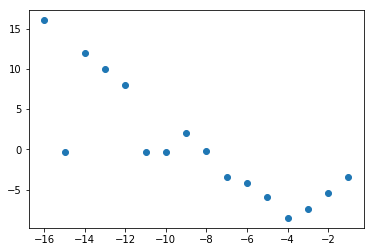
\includegraphics[scale=.5]{img/exercise1.png}
    \caption{ \( \log_{10}(h) \) vs. \( \log_{10}|error| \) }
\end{figure}
\end{solution}


\begin{problem}[Problem 2]
Use the formula in the previous exercise with \(h=0.2\), \(h=0.1\), and \(h=0.05\) to approximate \(u'' (x)\), where \(u(x) = \sin x\) and \(x = \pi / 6\).  Use one step of Richardson extrapolation, combining the results from \(h=0.2\) and \(h=0.1\), to obtain a higher order accurate approximation.  Do the same with the results from \(h=0.1\) and \(h=0.05\).  Finally do a second step of Richardson extrapolation, combining the two previously extrapolated values, to obtain a still higher order accurate approximation.  Make a table of the computed results and their errors.  What do you think is the order of accuracy after one step of Richardson extrapolation?  How about after two?
\end{problem}

\begin{solution}[Solution]
We expand,
\begin{align*}
    u(x+h) = u(x) + h u'(x) + \dfrac{h^2}{2!}u''(x) + \dfrac{h^3}{3!}u'''(x) + \dfrac{h^4}{4!}u^{(4)}(x) ... \\
    u(x-h) = u(x) - h u'(x) + \dfrac{h^2}{2!}u''(x) - \dfrac{h^3}{3!}u'''(x) + \dfrac{h^4}{4!}u^{(4)}(x) ... \\
\end{align*}

Thus,
\begin{align*}
    \dfrac{u(x+h)+u(x-h)-2u(x)}{h^2} &= \dfrac{2}{h^2}\left(\dfrac{h^2}{2!} u''(x) + \dfrac{h^4}{4!} u^{(4)}(x) + \dfrac{h^6}{6!}u^{(6)}(x) + \cO(h^8) \right) \\
    &= u''(x) + \dfrac{2h^2}{4!}u^{(4)}(x) + \dfrac{2h^4}{6!}u^{(6)}(x) + \cO(h^6)
\end{align*}

Call the left hand side \( \phi_0(h) \). Then, applying one step of Richardson extrapolation we have,
\begin{align*}
    \dfrac{4\phi_0(h/2)-\phi_1(h)}{3} &= u''(x) + \dfrac{1}{3}\dfrac{2}{6!}\left[4\dfrac{h^4}{2^4}-h^2\right] u^{(6)}(x) + \cO(h^6) \\
    &= u''(x) - \dfrac{h^4}{2\cdot 6!} u^{(6)}(x) + \cO(h^6)
\end{align*}

    Call the left hand side \( \phi_1(h) \). Applying an additional step gives,
\begin{align*}
    \dfrac{16\phi_1(h/2)-\phi_1(h)}{15} = \cO(h^6)
\end{align*}

We implement these computations in Python as,
\begin{lstlisting}
def fdq(u,x,h):
    return (u(x+h) + u(x-h) - 2*u(x))/h**2

x = np.pi/6
ans = -0.5

phi0 = fdq(np.sin,x,np.array([0.2,0.1,0.05]))
phi1 = [(4*phi0[1]-phi0[0])/3, (4*phi0[2]-phi0[1])/3]
phi2 = (16*phi1[1]-phi1[0])/15

out = np.append(phi0,np.append(phi1,phi2))
print(out)
print(out-ans)
\end{lstlisting}

The output is summarized in Table~\ref{richardson}.

    \begin{table}[H]\centering \tt
\begin{tabular}{|r|l|l|} \hline
    & {\rm value} & {\rm error } \\ \hline
    \( \phi_0(1/5) \) & -0.4983355539689565 & 1.6644460310435427e-03 \\
    \( \phi_0(1/10) \) & -0.4995834721974178 & 4.1652780258216726e-04 \\
    \( \phi_0(1/20) \) & -0.4998958420134868 & 1.0415798651319808e-04\\ \hline
    \( \phi_1(1/5) = [4\phi_0(1/10)-\phi_0(1/5)]/3 \) & -0.4999994449402383 &  5.5505976170877602e-07\\ 
    \( \phi_1(1/10) = [4\phi_0(1/20)-\phi_0(1/10)]/3 \) & -0.4999999652855098 & 3.4714490226850359e-08\\ \hline
    \( [16\phi_1(1/10)-\phi_1(1/5)]/15 \) & -0.4999999999751946 & 2.4805435483443716e-11 \\\hline
\end{tabular}
    \caption{Values of Richardson Extrapolation}
    \label{richardson}
\end{table}

We know the errors for \( \phi_0 \) and \( \phi_1 \) are \( \cO(h^4) \) and \( \cO(h^6) \) respectively.
\end{solution}


\begin{problem}[Problem 3]
Using Taylor series, derive the error term for the approximation
\[ u' (x) \approx \frac{1}{2h} [ -3 u(x) + 4 u(x+h) - u(x+2h) ] .\]
\end{problem}

\begin{solution}[Solution]
We expand,
\begin{align*}
    u(x+h) &= u(x) + h u'(x) + \dfrac{h^2}{2!}u''(x) + \dfrac{h^3}{3!}u'''(x) + \cO(h^4) \\
    u(x+2h) &= u(x) + 2h u'(x) + 4\dfrac{h^2}{2!}u''(x) + 8\dfrac{h^3}{3!}u'''(x) + \cO(h^4) 
\end{align*}

Thus,
\begin{align*}
    4u(x+h)-u(x+2h) &= (4-1)u(x) + (4-2)h u'(x) + (4-4)\dfrac{h^2}{2!}u''(x) + (4-8) \dfrac{h^3}{3!}u'''(x) + \cO(h^4) \\
    &= 3u(x) +2 h u'(x) - 4 \dfrac{h^3}{3!}u'''(x) + \cO(h^4)
\end{align*}

Then,
\begin{align*}
    \dfrac{1}{2h}[-3u(x)+4u(x+h) - u(x+2h)] &= \dfrac{1}{2h}\left[2hu'(x) - 4 \dfrac{h^3}{3!}u'''(x) + \cO(h^4) \right]
    = u'(x) - \dfrac{2h^2}{3!}u'''(x) + \cO(h^3)
\end{align*}

Therefore the error term to the above approximation is,
\begin{align*}
    - \dfrac{2h^2}{3!}u'''(x) + \cO(h^3)
\end{align*}
\end{solution}

\begin{problem}[Problem 4]
Consider a forward difference approximation for the second derivative of the form
    \[ u'' (x) \approx A u(x) + B u(x+h) + C u(x+2h) .\]
Use Taylor's theorem to determine the coefficients \(A\), \(B\), and \(C\) that give the maximal order of accuracy and determine what this order is.
\end{problem}

\begin{solution}[Solution]
We expand,
\begin{align*}
    u(x+h) &= u(x) + h u'(x) + \dfrac{h^2}{2!}u''(x) + \dfrac{h^3}{3!}u'''(x) + \cO(h^4) \\
    u(x+2h) &= u(x) + 2h u'(x) + 4\dfrac{h^2}{2!}u''(x) + 8\dfrac{h^3}{3!}u'''(x) + \cO(h^4) 
\end{align*}

Thus,
\begin{align*}
    Au(x) + Bu(x+h) + Cu(x+2h) 
    &= (A+B+C) u(x) + (B+2C)hu'(x) + (B+4C) \dfrac{h^2}{2!}u''(x)  \\
    & \hspace{3em}+ (B+8C)\dfrac{h^3}{3!}u'''(x) + \cO(h^4)(\cO(B)+\cO(C))
\end{align*}

We have three unknowns so we are only guaranteed to be able to satisfy three equations in these unknowns. We would like,
\begin{align*}
    A+B+C = B+2C= 0 && B+4C = 2/h^2
\end{align*}
so that the lowest order derivative remaining is \( u'' \).

We therefore require,
\begin{align*}
    A = \dfrac{1}{h^2} && B = -\dfrac{2}{h^2} && C = \dfrac{1}{h^2}
\end{align*}

We observe that any coefficients of the form \( B+2^k C \) will be nonzero for \( k\geq 2 \) and arbitrary \( x,h \). This means this is the best approximation we can make.

Thus, with this choice of coefficients,
\begin{align*}
    Au(x) + Bu(x+h) + Cu(x+2h) = \dfrac{1}{h^2}[u(x) - 2u(x+h) + u(x+2h)] = u''(x) + \cO(h)
\end{align*}

Therefore, this is an \( \cO(h) \) approximation.
\end{solution}

\begin{problem}[Problem 5]
Consider the two-point boundary value problem
\[ u'' + 2xu' - x^2 u = x^2 ,~~~u(0)=1,~~~u(1) = 0 .\]
Let \(h=1/4\) and explicitly write out the difference equations, using centered differences for all derivatives.
\end{problem}

\begin{solution}[Solution]
Write,
\begin{align*}
    x_0=0 && x_1 = 1/4 && x_2 = 2/4 && x_3 = 3/4 && x_4 = 1
\end{align*}

For \( j=1,2,3 \), we have,
\begin{align*}
    u'(x_j) \approx \dfrac{1}{2h}[u(x_{j+1})-u(x_{j-1})] 
    && u''(x_j) \approx \dfrac{1}{h^2}[u(x_{j+1})+u(x_{j-1})-2u(x_j)]
\end{align*}

Thus we have finite difference quotient,
\begin{align*}
    \dfrac{u_{j+1}+u_{j-1}-2u_j}{h^2} + 2x_j \dfrac{u_{j+1}-u_{j01}}{2h} - x_j^2 u_j
    &= x_j^2
\end{align*}

Writing \( u_j \) as the approximate values of \( u(x_j) \) for \( j=1,2,3 \), we have difference equations,
\begin{align*}
    \dfrac{u_2+u_0-2u_1}{1/4^2}+2 \left( \dfrac{1}{4} \right) \dfrac{u_2-u_0}{2\cdot 1/4} - \left( \dfrac{1}{4} \right)^2u_1
    = \left(\dfrac{1}{4}\right)^2 \\
    \dfrac{u_3+u_1-2u_2}{1/4^2}+2 \left( \dfrac{1}{2} \right) \dfrac{u_3-u_1}{2\cdot 1/4} - \left( \dfrac{2}{4} \right)^2u_2
    = \left(\dfrac{2}{4}\right)^2 \\
    \dfrac{u_4+u_2-2u_3}{1/4^2}+2 \left( \dfrac{3}{4} \right) \dfrac{u_4-u_2}{2\cdot 1/4} - \left( \dfrac{3}{4} \right)^2u_3 
    = \left(\dfrac{3}{4}\right)^2
\end{align*}

We group,
\begin{align*}
    (-2\cdot 16-1/16)u_1 + (16+1)u_2 = 1/16 - (16-1)u_0 \\
    (16-2)u_1 + (-2\cdot 16-1/4)u_2 + (16+2)u_3 = 1/4 \\
    (16-3)u_2 + (-2\cdot 16-9/16)u_3 = 9/16 - (16+3)u_4
\end{align*}

We simplify,
\begin{align*}
    - 513/16 u_1 + 17u_2 &= 1/16 - 15u_0 = -239/16 \\
    14u_1 - 129/4u_2  + 18u_3 &= 1/4 \\
    13u_2 - 521/16 u_3 &= 9/16-19u_4 = 9/16
\end{align*}

Rearranging and put in matrix form,
\begin{align*}
    \left[\begin{array}{rrr} -513 & 272 & 0 \\ 56 & -129 & 72 \\ 0 & 208 & -521 \end{array}\right]
    \left[\begin{array}{r}u_1 \\ u_2 \\ u_3\end{array}\right]
    =
    \left[\begin{array}{r} -239 \\ 1 \\ 9\end{array}\right]
\end{align*}

\end{solution}

\begin{problem}[Problem 6]
A rod of length 1 meter has a heat source applied to it and it eventually reaches a steady-state where the temperature is not changing.  The conductivity of the rod is a function of position \(x\) and is given by \(c(x) = 1 + x^2\).  The left end of the rod is held at a constant temperature of 1 degree.  The right end of the rod is insulated so that no heat flows in or out from that end of the rod.  This problem is described by the boundary value problem:
\[ \frac{d}{dx} \left( (1 + x^2 ) \frac{du}{dx} \right) = f(x) ,~~~ 
0 \leq x \leq 1 , \]
\[ u(0) = 1,~~~u'(1) = 0 . \]
\begin{enumerate}
\item[(a)] Write down a set of difference equations for this problem.
Be sure to show how you do the differencing at the endpoints.
[Note:  It is better {\bf not} to rewrite 
\(\frac{d}{dx} ( ( 1+ x^2 ) \frac{du}{dx} )\) as \((1 + x^2 ) u'' (x) + 2x u'(x)\);
leave the equation in the form above.]
\item[(b)] Write a MATLAB code to solve the difference equations. You can test your code on a problem where you know the solution by choosing a function \(u(x)\) that satisfies the boundary conditions and determining what \(f(x)\) must be in order for \(u(x)\) to solve the problem.  Try \(u(x) = (1-x )^2\).  Then \(f(x) = 2( 3 x^2 - 2 x + 1 )\). 
\item[(c)] Try several different values for the mesh size \(h\).  Based on your results, what would you say is the order of accuracy of your method?
\end{enumerate}
\end{problem}

\begin{solution}
\begin{enumerate}
    \item[(a)]
       For \( j=0 \) we have boundary condition,
        \begin{align*}
            x_0 = 0
        \end{align*}

        For \( j=1,2,...,m \) we use centered differences (with each derivative using spacing \( h/2 \)) to obtain an order \( h^2 \) approximation,

        We have,
        \begin{align*}
            u'(x) \approx \dfrac{1}{h}[u(x+\tfrac{h}{2})-u(x-\tfrac{h}{2})]
        \end{align*}
        
        Therefore,
        \begin{align*}
            (1+x^2)u'(x) \approx \dfrac{1+x^2}{h}[u(x+\tfrac{h}{2})-u(x-\tfrac{h}{2})]
        \end{align*}

        Finally,
        \begin{align*}
            \dfrac{d}{dx}[(1+x^2)u'(x)] &\approx
            \dfrac{1}{h} \left[ \dfrac{1+(x+\frac{h}{2})^2}{h}[u(x+h)-u(x)] - \dfrac{1+(x-\frac{h}{2})^2}{h}[u(x)-u(x-h)] \right] \\
            &= \dfrac{1}{h^2} \left[ (1+(x-\tfrac{h}{2})^2)u(x-h) - (2+(x+\tfrac{h}{2})^2+(x-\tfrac{h}{2})^2)u(x) + (1+(x+\tfrac{h}{2})^2)u(x+h) \right] \\
            &= \dfrac{1}{h^2} \left[ (1+(x-\tfrac{h}{2})^2)u(x-h) - 2(1+x^2+(\tfrac{h}{2})^2)u(x) + (1+(x+\tfrac{h}{2})^2)u(x+h) \right]
        \end{align*}

        We will introduce a point \( x_{m+2} \) in order to use a second order approximation for the Neumann boundary condition. We will never actually solve for \( u_{m+2} \).

        Thus, for \( j=1,2,...,m+1 \), we have difference equations,
        \begin{align*}
            f(x_j) = \dfrac{1}{h^2}[(1+(x_j-\tfrac{h}{2})^2)u_{j-1} - 2(1+x_j^2+(\tfrac{h}{2})^2)u_j + (1+(x_j+\tfrac{h}{2})^2)u_{j+1}    ] 
        \end{align*}

        In particular, note that for \( j=1 \) we write,
        \begin{align*}
            f(x_1)-\dfrac{1}{h^2}(1+(x_1-\tfrac{h}{2})^2))(1) = \dfrac{1}{h^2} [ -2(1+x_1^2+(\tfrac{h}{2})^2)u_{1} + (1+(x_1+\tfrac{h}{2})^2)u_{2} ]
        \end{align*}

        Finally, for \( j=m+1 \) we use the second order accurate centered difference equation,
        \begin{align*}
            \dfrac{1}{2h}[u_{m+2} - u_{m}] = 0
        \end{align*}
        
        Then \( u_{m+2} = u_{m} \). We substitute this into our equation above giving,
        \begin{align*}
            f(x_{m+1}) &= \dfrac{1}{h^2}[(1+(x_{m+1}-\tfrac{h}{2})^2)u_{m} - 2(1+x_{m+1}^2+(\tfrac{h}{2})^2)u_{m+1} + (1+(x_{m+1}+\tfrac{h}{2})^2)u_{m+2}    ] \\ 
            &= \dfrac{1}{h^2}[(1+(x_{m+1}-\tfrac{h}{2})^2)u_{m} - 2(1+x_{m+1}^2+(\tfrac{h}{2})^2)u_{m+1} + (1+(x_{m+1}+\tfrac{h}{2})^2)u_{m}    ] \\ 
            &= \dfrac{1}{h^2}[(2+(x_{m+1}-\tfrac{h}{2})^2 + (x_{m+1}+\tfrac{h}{2})^2))u_{m} - 2(1+x_{m+1}^2+(\tfrac{h}{2})^2)u_{m+1}   ] \\
            &= \dfrac{1}{h^2}[2(1+x_{m+1}^2+(\tfrac{h}{2})^2)u_{m} - 2(1+x_{m+1}^2+(\tfrac{h}{2})^2)u_{m+1}   ]
        \end{align*}


   \item[(b)] We implement this in Python (along with the loop for part (c)) as,
        \begin{lstlisting}
def exercise_6():
for m in [10,100,1000,10000]:
    h = 1/m
    h2 = h/2

    x = np.linspace(0,1,m+1)
    f = 2*(3*x[1:]**2-2*x[1:]+1) # start at x[1] since we evaluate for j=1,2,...

    f[0] -= (1+(x[1]-h2)**2)/h**2


    A = np.zeros((m,m))
    A[0,0:2] = [-2*(1+x[2]**2+h2**2),(1+(x[2]+h2)**2)]
    for j in range(2,m):
        A[j-1,j-2:j+1] = [(1+(x[j]-h2)**2),-2*(1+x[j]**2+h2**2),(1+(x[j]+h2)**2)]
    A[m-1,m-2:m] = [2*(1+x[j]**2+h2**2),-2*(1+x[j]**2+h2**2)]

    u = np.linalg.solve(A/h**2,f)
    print(h,np.max(u-(1-x[1:])**2))
        \end{lstlisting}

    \item[(c)]
        We loop over \( m\in\{10,10^2,10^3,10^4\} \) and print \( (h,\max_i\{u_i-(1-x_i^2)| i=1,2,...m+1\}) \). The results are summarized in Table~\ref{fdqerror}.

        \begin{table}[H]\centering\tt
            \begin{tabular}{|r|l|} \hline 
                \( h \) & \( \norm{u-u(x)}_\infty \) \\ \hline
                0.1 & 0.0306517881736 \\
                0.01 & 0.000279761901621 \\
                0.001 & 2.75753842277e-06 \\
                0.0001 & 2.72696144301e-08 \\ \hline
            \end{tabular}
            \caption{Mesh spacing vs error}
            \label{fdqerror}
        \end{table}

        As expected, since all of our difference quotients locally have error order \( h^2 \), the total error is order \( h^2 \). That is, for every order of magnitude decrease in \( h \), the error decreases by 2 orders of magnitude.

\end{enumerate}
\end{solution}

\end{document}
